\documentclass[10pt]{article}
\usepackage[utf8]{inputenc}
\usepackage{graphicx}
\usepackage{hyperref}
\graphicspath{{analysis/figures/}}
\begin{document}

\frontmatter




\title{FORMLÆRE}
\author{}
\date{Ei traktatform om korleis form oppstår}
\maketitle

\noindent
\includegraphics[width=\linewidth]{cover-stolar.png}





\chapter*{Innhald}

\tableofcontents

\chapter*{Føreord}


Kvifor har ting den forma dei har?
Svaret dei fleste designteoretiske tekstar gjev, er ein variant av Louis Sullivans «form follows function». Jan Michl har brukt det meste av ein akademisk karriere på å vise at dette svaret er feil. Ikkje berre upresist, men aktivt villfartande. Form følgjer ikkje funksjon. Form følgjer form. Kvar ny gjenstand er ein modifikasjon av ein eksisterande gjenstand, gjort av nokon som arbeider innanfor avgrensa moglegheiter og med avgrensa kunnskap om kva dei gjer. Michl rydda grunnen grundigare enn nokon før han. Han viste at den funksjonalistiske doktrinen ikkje berre var upresis, men at ho hindra oss i å sjå korleis formgjeving faktisk verkar.

George Kubler kom nærare. I The Shape of Time (1962) viste han at former ordnar seg i sekvensar, at kvar gjenstand er eit punkt i ein formell sekvens, og at somme punkt er «prime objects» som opnar nye sekvensar medan andre er replikasjonar. Kubler såg forma si historie som eit problem om posisjon og tid, ikkje om meining og bruk. Men han mangla eit apparat for å forklare kvifor sekvensane tek dei retningane dei gjer. Han skildra rørsla utan å identifisere kreftene.

Denne traktaten forsøkjer å gjere det Michl ikkje gjorde og Kubler ikkje kunne: å gje eit substrat-uavhengig rammeverk for korleis form oppstår. Ikkje kvifor ein bestemt stol ser ut som han gjer, men kva slags prosess som genererer alle former, inkludert stolar, inkludert bein, inkludert fuglereit, inkludert algoritmar. Svaret kan samanfattast i éi setning: Form er ein posisjon i eit rom bland moglege former, forma av samtidige seleksjonstrykk, navigert av aktørar på fleire skalaer.

Kva rammeverket ikkje kan seie. Traktaten handlar om posisjonar og krefter, ikkje om verdi. Ho kan forklare kvifor ein Wegner-stol og ein Monobloc okkuperer ulike posisjonar i same landskap. Ho kan ikkje seie noko om kvifor den eine er verdt å halde i handa og den andre ikkje er det. Estetisk dom ligg utanfor formsystemet, på same vis som etikk ligg utanfor logikken i Wittgensteins framstilling. Ikkje fordi det er uviktig, men fordi det ikkje let seg fange i proposisjonar. Ho seier heller ikkje noko om intensjon. Formgjevaren si oppleving av å skape, tvilerådinga, det brå gjennombrotet, den langsame tilnærminga, er usynleg i landskapsmodellen. Agenten navigerer; modellen registrerer berre den resulterende posisjonen. Innvendig liv er ikkje same sak som ytre spor.

Wittgenstein skriv at den som forstår han, erkjenner at setningane hans er meiningslause, og kastar stigen etter å ha klatra opp. Min stige er meir beskjeden: proposisjonane i denne traktaten er nyttige berre dersom formgjevaren, etter å ha lese dei, kan legge dei frå seg og navigere landskapet med same intuisjon som før, men no med ei forståing av kvifor intuisjonen verkar. Rammeverket skal ikkje erstatte handverket. Det skal vise handverket kva det allereie gjer. Dersom eg ikkje tek feil i dette, så har eg sagt noko om form som var sant før eg sa det, og som vil vere sant etter at desse orda er gløymd.

Oslo, 2026


\chapter*{Ordliste}




\textbf{Affordanse:} Dei formene eit materiale tilbyr og motset seg, i kraft av sine fysiske eigenskapar og dei produksjonsprosessane som er tilgjengelege. Avgjer kva formoperasjonar som er moglege (Gibson, 1979). [Def. i 2.6]




\textbf{Agensspektrum:} Agentar varierer i korleis dei best kan styrast: frå maskinvaremodifikasjon via settpunktomskriving og trening med belønning til kommunikasjon av grunnar. For kvart steg treng ein mindre kunnskap om systemets indre og meir kommunikasjon med systemet som heilskap. [Sjå 5.3]




\textbf{Agent:} Eit system definert av trippelet (mål, måling, justering). Krev korkje medvit, intensjon eller nervesystem. Krev berre funksjonell organisering: negativ tilbakekopling (Rosenblueth et al., 1943; Wiener, 1948). [Def. i 5.2]




\textbf{Formalgebra:} Mengda av former i eit euklidsk rom, utstyrt med operasjonane sum, differanse og produkt. Grunnlaget for formgrammatikken. [Def. i D4]




\textbf{Formgjevar:} Kvar instans av agens i formdomenet. Materialet er ein formgjevar. Marknaden er ein formgjevar. Handverkaren er ein formgjevar. Synonym med agent (def. 5.2) når konteksten er formgjeving. [Sjå 5.2, 6.1]




\textbf{Formgrammatikk:} Ein algebra over former i eit euklidsk rom, med reglar som opererer under innleiring: kvar regel fyrer for kvar førekomst av venstre side i noverande form, eventuelt transformert. Konstruksjonshistoria er irrelevant; berre den noverande forma avgjer kva reglar som kan fyre. Grammatikken spesifiserer kva som er mogleg; seleksjonstrykka avgjer kva som vert realisert. [Def. i 3.42, formelt i D4]




\textbf{Formrom (morphospace):} Mengda av alle moglege former innanfor ein gjeven klasse (ei gruppe objekt med same hovudfunksjon). Eit matematisk rom der kvar akse representerer ein målbar eigenskap. Kvar realisert gjenstand er eitt punkt i denne projeksjonen. [Def. i 1.2]




\textbf{Innleiring:} Ein euklidsk transformasjon som viser at éi form finst i ei anna, eventuelt rotert, flytta eller skalert. Innleiringa er ein eigenskap ved den noverande forma, uavhengig av korleis ho vart konstruert. Avgjer kva generative operasjonar som er tilgjengelege for ein agent. [Def. i D4, kopla til D8 og T6]




\textbf{Kanalisering:} Graden av robustheit til ein form mot forstyrringar. Målt som brattleiken på dalveggane i landskapet. Bratte veggar: stabil stil. Flate veggar: ustabil (Waddington, 1957). [Def. i 3.3]




\textbf{Klasse:} Ei gruppe objekt som deler same hovudfunksjon. Klassen definerer formrommet. [Def. i 1.2]




\textbf{Kognitiv lyskjegle:} Den romleg-temporale regionen ein agent kan representere og påverke. Storleiken avheng av signalfarten i mediet. Avgrensinga gjeld ikkje berre rekkjevidda, men oppløysinga: kva intern struktur agenten kan oppdage i ei form (Fields \& Levin, 2022). [Def. i 5.5, 5.52]




\textbf{Projeksjon:} Avbildinga av ei form inn i formrommet gjennom eit val av aksar. Projeksjonen er naudsynt for empirisk testing, men tapsbringande: forma er rikare enn kvar endeleg mengd målingar kan fange. [Def. i 1.21]




\textbf{Seleksjonstrykk:} Ein faktor som endrar sannsynlegheitsfordelinga over formrommet. Ikkje ein regel som dikterer éi form, men ein gradient som gjer visse former meir sannsynlege enn andre. [Def. i 2.1]




\textbf{Substrat:} Det fysiske, algoritmiske eller sosiale systemet som realiserer agensen. Formrommet er substrat-uavhengig: posisjonen er den same uavhengig av korleis objektet vart laga (Turing, 1950; Levin, 2022). [Def. i 5.22]




\textbf{Tilpassingslandskap:} Grafen til den aggregerte verknaden av alle samtidige seleksjonstrykk over formrommet. Haugane er stabile posisjonar der kvar lita endring gjev dårlegare tilpassing; dalane er posisjonar ingen selekterer (Wright, 1932; Waddington, 1957). [Def. i 3.1]


Proposisjonane er haldne opp mot eit empirisk materiale beståande av om lag 2 300 europeiske stolar (1280–2024) frå Nasjonalmuseet og Victoria and Albert Museum. Tala tener som illustrasjonar, ikkje som premissar.



\textbf{Kvar proposisjon er utstyrt med ein superscript som indikerer logisk status:} d = definisjon, a = postulat, t = teorem, o = observasjon, i = illustrasjon. Kvart postulat er knytt til eit eksplisitt falsifiseringsvilkår. Michl har demonstrert at «form følgjer funksjon» kollapsa fordi formelen var logisk utilgjengeleg for falsifisering. Denne traktaten lukkast berre i den grad ho let seg fei




\mainmatter





\chapter*{1.~~Form er ein posisjon i eit rom av moglegheiter}




\noindent\textbf{1.1}\textsuperscript{\textit{o}}~~Alt som har form, har den forma det har og ikkje ei anna. At det har nettopp denne forma, når andre var moglege, krev ei forklaring. Forklaringa kan ikkje ligge i forma sjølv. Ho må ligge i tilhøvet mellom forma og dei andre formene som var moglege men ikkje vart realiserte.




\noindent\textbf{1.2}\textsuperscript{\textit{d}}~~Formrommet til ein klasse er mengda av alle moglege former gjenstander i denne klassen kan realisere. Klassen er definert av hovudfunksjonen. Kvar realisert gjenstand er eitt punkt i dette rommet.




\noindent\textbf{1.21}\textsuperscript{\textit{d}}~~Det empiriske formrommet er ein projeksjon. Projeksjonen er naudsynt for empirisk testing, men tapsbringande: forma er rikare enn kvar endeleg mengd målingar kan fange.




\noindent\textbf{1.22}\textsuperscript{\textit{d}}~~Same form kan dekomponerast i ulike delformer avhengig av kva operasjonar ein utfører. Valet av aksar avgjer kva klynger, grenser og tomrom analysen kan registrere.




\noindent\textbf{1.3}\textsuperscript{\textit{d}}~~Formrommet har tre regionar: dei busette, dei opne og dei forbodne. Dei busette er realiserte posisjonar. Dei opne er moglege men urealiserte. Dei forbodne er fysisk umoglege.




\noindent\textbf{1.31}\textsuperscript{\textit{o}}~~Grensa mellom dei opne og dei forbodne er ein funksjon av tilgjengeleg teknologi. Det som var forbode i går, kan vere ope i dag.




\noindent\textbf{1.32}\textsuperscript{\textit{o}}~~Ei open region kan artikulerast som ein uavgjord proposisjon: «det finst ein stol utan bein» namngjev ein posisjon som korkje er realisert eller forboden. Skilnaden er empirisk, ikkje logisk.




\noindent\textbf{1.4}\textsuperscript{\textit{o}}~~Formrommet er ikkje uniformt busett. Dei realiserte formene aggregerer i klynger kring spesifikke posisjonar, med tomme regionar mellom seg. Denne ikkje-uniformiteten krev forklaring.




\noindent\textbf{1.5}\textsuperscript{\textit{t}}~~Sidan fordelinga av former ikkje er tilfeldig, må det finnast faktorar som favoriserer visse posisjonar framfor andre. Å identifisere desse faktorane er målet for det fylgjande.




\noindent\textbf{1.6}\textsuperscript{\textit{d}}~~Ein einskild form er eit punkt. Ein stil er ei klynge. Ein tradisjon er ein stig av ordna punkt over tid, der kvar ny gjenstand er ein modifikasjon av ein eksisterande.




\noindent\textbf{1.7}\textsuperscript{\textit{t}}~~Formrommet er substrat-uavhengig. Same posisjon kan okkuperast av ein handverkar, ein fabrikk eller ein algoritme. Posisjonen er invariant; vegen dit er lokal.




\noindent\textbf{1.71}\textsuperscript{\textit{t}}~~Substrat-uavhengigheita gjeld posisjonen, ikkje navigasjonen. Form fungerer som den induktive premissen for vidare form: kvar ny gjenstand startar frå ein eksisterande, gjord av nokon som arbeider innanfor avgrensa moglegheiter og med avgrensa kunnskap om kva dei gjer.







\chapter*{2.~~Ikkje alle posisjonar er like sannsynlege}




\noindent\textbf{2.1}\textsuperscript{\textit{d}}~~Eit seleksjonstrykk er ein faktor som endrar sannsynlegheitsfordelinga over formrommet. Ikkje ein regel som dikterer éi form, men ein gradient som gjer visse posisjonar meir sannsynlege enn andre.




\noindent\textbf{2.11}\textsuperscript{\textit{t}}~~Eit seleksjonstrykk åleine determinerer ikkje ein posisjon. Det avgrensar kvar posisjonen \textit{ikkje} kan vere. Form er det som vert att når alle seleksjonstrykk har utelukka det dei kan utelukke.




\noindent\textbf{2.12}\textsuperscript{\textit{t}}~~Eit trykk som ikkje utelukkar nokon region, er ikkje eit trykk; det er ein tom kategori. Eit trykk som utelukkar alle regionar unntatt éin, er ikkje eit trykk; det er ein determinisme. Dei trykka vi observerer ligg mellom desse ytterpunkta.




\noindent\textbf{2.2}\textsuperscript{\textit{a}}~~For kvar funksjonell klasse verkar det alltid meir enn eitt seleksjonstrykk samstundes. Einsidige forklaringar av form er alltid ufullstendige.




\noindent\textbf{2.21}\textsuperscript{\textit{t}}~~Dersom berre eitt trykk verka, ville alle former i klassen enten vere identiske eller tilfeldig fordelte langs den eine aksen. Den observerte ikkje-uniformiteten med variasjon i fleire retningar tyder at fleire uavhengige trykk verkar samstundes.




\noindent\textbf{2.3}\textsuperscript{\textit{a}}~~For minst eitt par av seleksjonstrykk peikar gradientane i motstridande retningar i minst éin region av formrommet.




\noindent\textbf{2.4}\textsuperscript{\textit{t}}~~Av 2.2 og 2.3: sidan fleire uavhengige trykk verkar og dreg i ulike retningar, kan ikkje alle verte optimalt tilfredsstilte. Kvar realisert form er eit kompromiss. Eit kompromiss er ikkje ein svakheit; det er den einaste moglege balansen under dei vilkåra som rådde.




\noindent\textbf{2.41}\textsuperscript{\textit{t}}~~Sidan det finst fleire gyldige kompromiss, er skilnaden mellom to former ikkje ein feil, men eit uttrykk for at kreftene kan balanserast på meir enn éin måte.




\noindent\textbf{2.5}\textsuperscript{\textit{t}}~~Funksjonen definerer klassen og med det formrommet. Innanfor klassen er funksjonen konstant. Det som er konstant har null varians og ber null informasjon om kvifor éi bestemt form vart realisert framfor ei anna. All observert formvariasjon under konstant funksjon er driven av dei andre seleksjonstrykka.




\noindent\textbf{2.6}\textsuperscript{\textit{d}}~~Materialaffordansen er dei operasjonane eit materiale tilbyr og motset seg under gjevne kostnads- og tilgjengelegheitsavgrensingar. Signaturen er probabilistisk: repertoaret bind sannsynsfordelinga, ikkje det einskilde objektet.




\noindent\textbf{2.61}\textsuperscript{\textit{o}}~~Signaturen er latent. Det teoretiske repertoaret slår ikkje nødvendigvis ut i observerbar geometri. Materialet er til stades, men algebraen manglar. Det som endrar seg over tid er ikkje materialet, men kva operasjonar som er praktisk tilgjengelege.




\noindent\textbf{2.62}\textsuperscript{\textit{o}}~~Latensen kan vere lang. Stål var tilgjengeleg i hundreår før den fyrste røyrstolen; materialet fanst, men operasjonen som kunne utnytte det, fanst ikkje. Formhistoria er langsamare enn materialhistoria.




\noindent\textbf{2.63}\textsuperscript{\textit{o}}~~Eit nytt materiale arvar difor formspråket til det substratet det erstattar, heilt til eigne affordansar pressar det ut i nye regionar av formrommet.




\noindent\textbf{2.7}\textsuperscript{\textit{o}}~~Ein samlevariabel korrelert med alle samtidige seleksjonstrykk bør predikere formvariasjon betre enn kvart einskildtrykk. Stilperiode er ein slik samlevariabel. Han er ikkje ein forklaring; han er ein proxy som absorberer alle samtidige trykk i éin etikett. Stilkategoriane beskriv kvar vandringa stansa. Dei forklarer ikkje kvifor.







\chapter*{3.~~Seleksjonstrykka produserer eit landskap over formrommet}




\noindent\textbf{3.1}\textsuperscript{\textit{d}}~~Tilpassingslandskapet er den aggregerte verknaden av alle samtidige seleksjonstrykk over formrommet. Kvar posisjon har ein verdi: kor godt forma tilfredsstiller alle verksame trykk samstundes.




\noindent\textbf{3.11}\textsuperscript{\textit{o}}~~Kvart seleksjonstrykk bidreg til landskapet med ein vekt som varierer over tid. Vektene er ikkje frie parametrar; dei er empirisk tilgjengelege som samvariasjonen mellom kvart trykk og den observerte fordelinga, betinga på alle andre trykk.




\noindent\textbf{3.12}\textsuperscript{\textit{o}}~~Landskapet er retrospektivt rekonstruerbart. For eit gjeve tidspunkt kan vektene estimerast frå dei realiserte formene i ein temporal nærleik. Det er lokalt prediktivt: det predikerer kva regionar som har høgast sannsynlegheit for neste okkupasjon, ikkje kva einskildform som vert realisert.




\noindent\textbf{3.13}\textsuperscript{\textit{o}}~~Prediksjonshorisonten er ein funksjon av landskapets endringsrate. I periodar med stase er prediksjonen lang; i bifurkasjonar kort. At prediksjonen er avgrensa, er ein eigenskap ved modellen, ikkje ein mangel.




\noindent\textbf{3.2}\textsuperscript{\textit{t}}~~Av 2.2, 2.3 og 3.1: tilpassingsfunksjonen har generisk fleire lokale maksima. Landskapet har difor fleire haugar. Ein haug er ein posisjon der kvar lita endring gjev dårlegare tilpassing. Former samlar seg på haugane. Dalar er posisjonar ingen selekterer.




\noindent\textbf{3.3}\textsuperscript{\textit{d}}~~Stabilitetsgraden til ein haug er brattleiken på dalveggane. Bratte veggar tyder kanalisering: forma er robust mot forstyrringar, slik eit embryo er robust mot genetisk variasjon. Flate veggar tyder ustabilitet.




\noindent\textbf{3.31}\textsuperscript{\textit{t}}~~Nokre seleksjonstrykk er sterkare enn andre. Dei sterkaste kanaliserer formrommet i få retningar. Hierarkiet av trykk produserer eit hierarki av kanalar: grove kanalar fyrst, finare innanfor dei grove.




\noindent\textbf{3.4}\textsuperscript{\textit{d}}~~Ein stil er ei klynge av realiserte former kring same haug. At ein stil er ei klynge, ikkje ein kategori, forklarer kvifor stilar har uskarpe grenser: grensa mellom to klynger i eit kontinuerleg rom er naudsynleg diffus. Stilperiodar er gradientar, ikkje topologiske klynger.




\noindent\textbf{3.5}\textsuperscript{\textit{t}}~~Formgjeving konstruerer ikkje landskapet. Landskapet er gjeve av vilkåra. Å oppdage ein haug er ikkje å skape han.




\noindent\textbf{3.6}\textsuperscript{\textit{t}}~~Ei form som dukkar opp uavhengig i tradisjonar utan kontakt, er sterkt prov for at haugen er ein eigenskap ved landskapet, ikkje ved nokon einskild tradisjon. Konvergensen forklarer seg sjølv: same vilkår, same gradient, same haug.







\chapter*{4.~~Landskapet er dynamisk}




\noindent\textbf{4.1}\textsuperscript{\textit{a}}~~Seleksjonstrykka er ikkje konstante over tid. Ein ny teknologi flyttar grensa for det forbodne i formrommet. Ein ny marknad rekonfigurerer kva som vert belønna. Eit nytt materiale utvidar mengda av moglege operasjonar.




\noindent\textbf{4.2}\textsuperscript{\textit{t}}~~Av 3.1 og 4.1: landskapet er ein dynamisk flate. Haugar kan stige, søkke, flytte seg, bifurkere eller koalescere. Ein posisjon som var optimalt tilpassa under eitt sett av vilkår, kan i neste augeblink vere suboptimal.




\noindent\textbf{4.3}\textsuperscript{\textit{o}}~~Endringa er diskontinuerleg. Lange periodar med stase vert avbrotne av brå topologiske skifte: ein eksplosiv radiasjon inn i ein nyopna region, fylgd av gradvis konvergens mot nye attraktorar.




\noindent\textbf{4.4}\textsuperscript{\textit{o}}~~Landskapet har minne. Kvar realisert form etterlet eit spor som modifiserer seleksjonstrykka for den neste. Forma og landskapet endrar kvarandre gjensidig. All formgjeving er omformgjeving: agenten startar aldri frå ein tom posisjon.




\noindent\textbf{4.5}\textsuperscript{\textit{o}}~~Formrommet ekspanderer kumulativt. Nye regionar vert busette; gamle vert sjeldan heilt forlate.




\noindent\textbf{4.6}\textsuperscript{\textit{o}}~~Materialstraumar er ein hovudmekanisme for landskapsendring. Kvart nytt materiale opnar nye regionar og stengjer andre.




\noindent\textbf{4.7}\textsuperscript{\textit{i}}~~Når eitt seleksjonstrykk vert dominant, kollapsar landskapet til éin attraktor. Ikkje berre materialrommet krympar, men formrommet sjølv. Eitt trykk som overkøyrer alle andre er ikkje ei forklaring av form; det er eit fråvær av forklaring.







\chapter*{5.~~Det finst agentar som responderer på landskapet}




\noindent\textbf{5.1}\textsuperscript{\textit{a}}~~For kvar funksjonell klasse finst det minst éin system som navigerer tilpassingslandskapet via negativ tilbakekopling. Eit slikt system kallar vi ein agent.




\noindent\textbf{5.2}\textsuperscript{\textit{d}}~~Ein agent er definert av trippelet måltilstand, avstandsmåling, justering. Definisjonen krev tilbakekopling. Ho krev korkje medvit, intensjon eller nervesystem; ho krev berre funksjonell organisering. Eit system som ikkje treng å vite kva det er laga av for å navigere mot eit mål, er ein agent uavhengig av kva det er laga av.




\noindent\textbf{5.21}\textsuperscript{\textit{t}}~~Eit system utan tilbakekopling er ikkje ein agent. Ein stein som rullar nedover ei skråning manglar justeringsmekanisme: rørsla hans responderer ikkje på nokon avstand til nokon måltilstand. Grensa mellom agent og ikkje-agent går ved informasjonsflyt. Ein flod som eroderer er ikkje ein agent; ein planaria som regenererer er det.




\noindent\textbf{5.22}\textsuperscript{\textit{t}}~~Definisjonen er generell. Ho fangar alt frå ein termostat til ein designar. Diskriminerande kraft kjem ikkje frå definisjonen, men frå graderinga.




\noindent\textbf{5.23}\textsuperscript{\textit{o}}~~Agentar skil seg i tre målbare eigenskapar: kor mykje av formrommet dei kan representere, kor rask tilbakekoplinga er, og kor djup læringsevna er.





\includegraphics[width=\linewidth]{fig-5.23-agentar.png}





Definisjonen er ikkje vakuøs; ho er stratifisert.




\noindent\textbf{5.24}\textsuperscript{\textit{o}}~~Agens utgjer eit spektrum. Agentar varierer i korleis dei best kan styrast: frå maskinvaremodifikasjon via settpunktomskriving og trening med belønning til kommunikasjon av grunnar. For kvart steg treng ein mindre kunnskap om systemets indre og meir interaksjon med systemet som heilskap.




\noindent\textbf{5.3}\textsuperscript{\textit{t}}~~Agenten responderer ikkje på forma, men på landskapet. Måltilstanden er ikkje ein posisjon agenten oppfinnar; det er ein haug i landskapet agenten oppdagar.




\noindent\textbf{5.31}\textsuperscript{\textit{t}}~~Agenten treng ikkje å forstå landskapet for å navigere det. Det er tilstrekkeleg å registrere den lokale gradienten. Navigasjonskompetanse krev ikkje kartografi.




\noindent\textbf{5.4}\textsuperscript{\textit{d}}~~Den kognitive lyskjegla til ein agent er den delmengda av formrommet han kan representere og påverke. Det som ligg utanfor lyskjegla, er kausalt utilgjengeleg.




\noindent\textbf{5.41}\textsuperscript{\textit{o}}~~Lyskjeglene varierer i skala: frå cellulær fysiologi over minutt til designtradisjonar over hundreår.




\noindent\textbf{5.42}\textsuperscript{\textit{o}}~~Lyskjegla avgrensar oppløysinga: kva delformer ein agent kan identifisere, avgjer kva transformasjonar som er tilgjengelege. Barnet, snikkaren og algoritmen dekomponerer same form i ulike operasjonelle einingar.




\noindent\textbf{5.43}\textsuperscript{\textit{t}}~~Ein agent oppdagar ikkje former; han oppdagar affordansar. Ein affordans er ein lokal eigenskap ved landskapet som berre er synleg innanfor lyskjegla. Å utvide lyskjegla er å gjere latente affordansar synlege.




\noindent\textbf{5.44}\textsuperscript{\textit{d}}~~Fem operasjonar modifiserer lyskjegla:





\includegraphics[width=\linewidth]{fig-5.44-lyskjegle.png}





Operasjonane føreset berre kausal rekkevidd og tilbakekopling.




\noindent\textbf{5.45}\textsuperscript{\textit{o}}~~C-K-teorien formaliserer den intensjonale navigasjonen som veksling mellom konseptrom (C) og kunnskapsrom (K). Dei fire C-K-operatorane svarar til restriksjonar av lyskjegleoperasjonane:





\includegraphics[width=\linewidth]{fig-5.45-ck.png}





C-K er det proposisjonslogiske spesialtilfellet av ein meir generell struktur. Lyskjegla krev ikkje proposisjonar; ho krev berre kausal rekkevidd.




\noindent\textbf{5.5}\textsuperscript{\textit{o}}~~Navigasjonskompetanse er akkumulert. Kvar realisert form utvidar agentens lyskjegle. Læring er den temporale utvidinga av agentens tilgjengelege formrom.




\noindent\textbf{5.51}\textsuperscript{\textit{t}}~~Læring er hierarkisk: frå enkel navigasjon via strategiskifte til restrukturering av sjølve formrommet. Læring, biologisk seleksjon og bayesiansk inferens er isomorfe operasjonar i ulike substrat; dei minskar alle avstanden mellom modell og verd.




\noindent\textbf{5.6}\textsuperscript{\textit{d}}~~Blant agentens kompetansar er evna til å operere direkte på geometri. Mengda av former i eit euklidsk rom, utstyrt med operasjonane sum og differanse, utgjer ein formalgebra. Formalgebraen er grunnlaget for det generative systemet.




\noindent\textbf{5.61}\textsuperscript{\textit{d}}~~Ein formgrammatikk er eit sett reglar som opererer direkte på geometri: finn denne delforma i den noverande forma; erstatt ho med denne andre. Kvar regel er definert under innleiring: ei delform kan identifiserast i den noverande forma uavhengig av korleis ho vart bygd. Reglane ser; dei hugsar ikkje.




\noindent\textbf{5.62}\textsuperscript{\textit{d}}~~Reglane transformerer former på fem måtar:





\includegraphics[width=\linewidth]{fig-5.62-grammatikk.png}


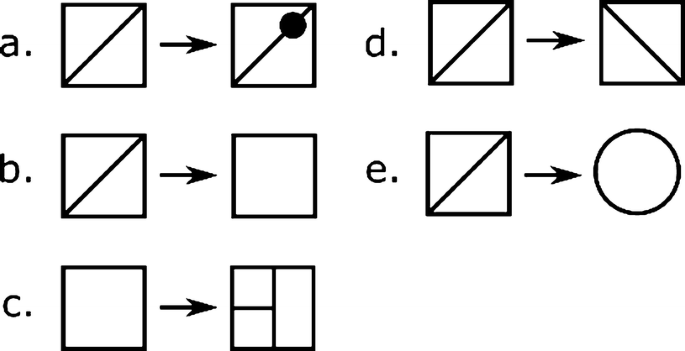
\includegraphics[width=0.78\linewidth]{shape_grammar_fig1.png}





\noindent\textbf{5.63}\textsuperscript{\textit{t}}~~Av 5.61: forma sjølv avgjer kva reglar som kan fyre. Den noverande geometrien er den einaste premissen. Konstruksjonshistoria er irrelevant.




\noindent\textbf{5.64}\textsuperscript{\textit{d}}~~Grammatikken genererer ein naboskap for kvar form: mengda av alle former som kan nåast ved éin operasjon. Naboskapen er formens lokale moglegheitsrom.




\noindent\textbf{5.641}\textsuperscript{\textit{t}}~~Naboskapen er ikkje symmetrisk. At du kan kome dit, tyder ikkje at du kan kome attende. Formrommet har ein retta struktur.




\noindent\textbf{5.65}\textsuperscript{\textit{t}}~~Kombinasjonen av to former kan framkalle delformer ingen av dei inneheldt åleine. Same form, ulike dekomposisjonar: ikkje fordi forma er tvetydig, men fordi ho er rikare enn kvar einskild operasjon som produserte ho.




\noindent\textbf{5.66}\textsuperscript{\textit{t}}~~Grammatikken spesifiserer kva som er mogleg; seleksjonstrykka avgjer kva som vert realisert. Grammatikken og landskapet møtest i agentens val: naboskapen gjev moglegheitene, landskapet gjev kvar moglegheit ein verdi, agenten aktualiserer den forma som tilfredsstiller gradienten.




\noindent\textbf{5.67}\textsuperscript{\textit{t}}~~Av 5.42 og 5.61: sidan lyskjegla avgjer kva innleiringar agenten kan oppdage, og sidan innleiringa avgjer kva reglar som kan fyre, er den generative kapasiteten avgrensa av lyskjegla. To agentar med same grammatikk men ulike lyskjeglar produserer ulike former.




\noindent\textbf{5.7}\textsuperscript{\textit{o}}~~Materialet deltek ikkje berre gjennom motstand. Det er ein agent av null-orden: det navigerer ikkje mot ein måltilstand, men det utelukkar posisjonar og favoriserer andre gjennom sine affordansar. Materialet gjev landskapet sin topografi.




\noindent\textbf{5.71}\textsuperscript{\textit{i}}~~Ein planaria navigerer morforommet via bioelektriske gradientar. Ein handverkar navigerer formrommet via taktil tilbakemelding. Ein diffusjonsmodell navigerer eit latent rom via denoising. Substrata er ulike; strukturen er identisk.







\chapter*{6.~~Forma oppstår mellom agentane}




\noindent\textbf{6.1}\textsuperscript{\textit{t}}~~Av 2.2 og 5.1: sidan meir enn eitt seleksjonstrykk alltid verkar, og sidan ulike agentar responderer på ulike trykk, er kvar realisert form eit poly-agentisk kompromiss. Materialaffordansen, reiskapen, marknaden og kulturen utgjer uavhengige gradientar. Ingen einskild agent dikterer den resulterande morfologien; ho emergerer i skjeringspunktet mellom dei, som ein posisjon ingen del kunne ha navigert mot åleine.




\noindent\textbf{6.2}\textsuperscript{\textit{t}}~~Kvart hierarkisk nivå er ein kompetent problemløysar innanfor sin eigen lyskjegle. Dei lågare komponentane navigerer etter lokale gradientar, men bidreg samstundes til mål dei sjølve manglar kapasitet til å representere. Reduksjonisme og holisme er komplementære skildringsnivå; begge er sanne, men ingen er tilstrekkeleg åleine.




\noindent\textbf{6.3}\textsuperscript{\textit{t}}~~Av 6.1 og 5.66: sjølv når éin agent har nominell kontroll, avgjer landskapet kva reglar som faktisk fyrer. Agenten vel frå naboskapen; landskapet filtrerer naboskapen. Kontrollen er alltid delt.




\noindent\textbf{6.31}\textsuperscript{\textit{o}}~~Kommunikasjonen mellom agentar er avgrensa av ein endeleg bandbreidde. Ved låg bandbreidde er navigasjonen grov og stokastisk; ved høg bandbreidde kan forma artikulerast gjennom eksplisitt spesifikasjon.




\noindent\textbf{6.32}\textsuperscript{\textit{t}}~~Det finst eit byttetilhøve mellom bandbreidde og uavhengigheit. Tett kopla agentar konvergerer mot eit felles representasjonsformat som avgrensar kva regionar dei kan utforske. Lauskopla agentar oppretheld kognitiv autonomi, men koordinerer dårlegare.




\noindent\textbf{6.33}\textsuperscript{\textit{o}}~~Bandbreidda har ein temporal dimensjon i form av latens. Ved låg latens er sanntidskoordinering mogleg; ved høg latens må kvar agent operere på ein intern modell av dei andre agentane sin framtidige tilstand. Koordineringa er då berre so presis som modellens adekvatheit.




\noindent\textbf{6.4}\textsuperscript{\textit{o}}~~Når koplinga mellom agentar er robust, emergerer eit overordna system med større lyskjegle og meir samansette mål. Ved brot i samanbindinga krympar systemet; ein del som frikoplar seg frå nettverket følgjer berre eigne, kortsiktige gradientar.




\noindent\textbf{6.41}\textsuperscript{\textit{t}}~~Når samanbindinga er tilstrekkeleg tett til at heilskapen realiserer ein eigen tilbakekoplingssyklus, vert heilskapen sjølv ein agent etter definisjonen i 5.2. Skiljet mellom ein aggregering av agentar og ein einskild agent er funksjonelt, ikkje ontologisk.




\noindent\textbf{6.42}\textsuperscript{\textit{o}}~~Eit multi-agent-system kan oppnå metastabilitet på tvers av fleire skalaer utan at nokon einskild skala er fullt optimalisert. Denne stabiliteten let tradisjonar persistere gjennom fluktuasjonar som ville ha utsletta delane deira om dei opererte i isolasjon.




\noindent\textbf{6.5}\textsuperscript{\textit{t}}~~Stilar og tradisjonar er deskriptive mellomkonstruksjonar utan kausal kraft. Dei skildrar dei punkta i formrommet der vandringa mellombels har stansa. Å formgje «i ein stil» er ein logisk feil: det er å imitere eit statistisk symptom utan å forstå dei seleksjonstrykka som genererte klynga i utgangspunktet.




\noindent\textbf{6.6}\textsuperscript{\textit{o}}~~Nyhetsraten i formrommet er ein funksjon av det tilstøytande moglege: kvar realisert form opnar nye regionar av naboskapen som ikkje fanst før. Det moglege veks med det realiserte.







\chapter*{7.~~Ingen form er endeleg}




\noindent\textbf{7.1}\textsuperscript{\textit{t}}~~Av 2.4 og 4.1: sidan seleksjonstrykka endrar seg, vil kvar realisert balanse med tida verte suboptimal. Posisjonen som var optimalt tilpassa under eitt sett av vilkår, er det ikkje under det neste. Kvar realisert form er gyldig berre for dei vilkåra som rådde i det augeblinket ho vart aktualisert.




\noindent\textbf{7.2}\textsuperscript{\textit{t}}~~Dei mest robuste tradisjonane er ikkje dei rigide, men dei med høgast agensstratifisering: fleire uavhengige tilpassingsmekanismar på fleire skalaer gjev raskare respons når landskapet endrar seg.




\noindent\textbf{7.3}\textsuperscript{\textit{o}}~~Det einaste varige er den generative strukturen: formrommet, seleksjonstrykka, landskapet, agentane. Formene i seg sjølve er flyktige spor; grammatikken er stabil.




\noindent\textbf{7.4}\textsuperscript{\textit{o}}~~Dette rammeverket er ikkje ein ontologisk påstand om kva form er. Det er eit koordinatsystem for spesifikasjon. At strukturen er substrat-uavhengig er eit teikn på fruktbarheit, ikkje eit prov for sanning.




\noindent\textbf{7.5}\textsuperscript{\textit{o}}~~Agenten som skildrar formverda er sjølv ein del av ho. Det finst ingen arkimedisk punkt på utsida. Ei formlære er aldri transcendent; ho er alltid lokal og situert.




\noindent\textbf{7.6}\textsuperscript{\textit{o}}~~Å gje form er: å definere kva måltilstand materien skal navigere mot; å velje kva krefter som skal utgjere landskapet; å utvide agentens kognitive lyskjegle slik at latente affordansar vert synlege; å akseptere at forma emergerer mellom agentane; å leggje til rette for vilkåra som dei kompetente delane opererer under.




\noindent\textbf{7.7}\textsuperscript{\textit{o}}~~Formverda er alt som er tilfelle. Tilpassingslandskapet er alt som verkar. Navigasjonen er utan slutt.




\noindent\textbf{7.8}\textsuperscript{\textit{o}}~~Denne traktaten er sjølv ein posisjon i eit formrom. Stigen vert ikkje kasta; ho vert kalibrert. At teksten kan fellast, er garantien for hennar gyldigheit.


\appendix
\chapter*{Formell spesifikasjon}


\section*{A.1~~Notasjon}





\noindent\textbf{c}~~ein klasse




\noindent\textbf{x}~~ei form




\noindent\textbf{p}~~eit seleksjonstrykk




\noindent\textbf{A}~~ein agent




\noindent\textbf{G}~~ein grammatikk




\noindent\textbf{t}~~eit tidspunkt


π : Shape \msym{→} \msym{ℝ}ⁿ: morforomprojeksjonen


\noindent\textbf{L(G)}~~språket (mengda av alle former) ein grammatikk G genererer




\noindent\textbf{H}~~Shannon-entropi




\noindent\textbf{I}~~gjensidig informasjon




\noindent\textbf{Cov}~~kovarians




\section*{A.3~~Definisjonar}





\noindent\textbf{D1}~~(Formrom, prop. 1.2)




Morphospace(c) := \{ π(x) : x \msym{∈} c \} \msym{⊆} \msym{ℝ}ⁿ




\noindent\textbf{D2}~~(Seleksjonstrykk, prop. 2.1)




p : \msym{ℝ}ⁿ \msym{→} \msym{ℝ}




\noindent\textbf{D3}~~(Tilpassingslandskap, prop. 3.1)




Landscape(c, t) := Σᵢ wᵢ(t) \msym{·} pᵢ




\noindent\textbf{D4}~~(Formalgebra og formgrammatikk, prop. 3.42)




Lat S vere ei mengd av former i eit euklidsk rom Eⁿ, utstyrt med operasjonar og lukka under den euklidske transformasjonsgruppa Trans(Eⁿ):




s₁ + s₂ (sum)




s₁ − s₂ (differanse)




(snittet s₁ \msym{·} s₂ := s₁ − (s₁ − s₂) er ein avleidd, ikkje primitiv, operasjon)




Ein innleiring av a i s er ein transformasjon τ \msym{∈} Trans(Eⁿ) slik at τ(a) \msym{≤} s.




Ein formgrammatikk er eit trippel SG = (S, R, ω) der R = \{ rᵢ : (aᵢ, bᵢ) \}, med regelapplikasjon:




s \msym{→} (s − τ(aᵢ)) + τ(bᵢ)




L(SG) = \{ s \msym{∈} S : ω \msym{→}* s ved bruk av reglar i R \}




\noindent\textbf{D5}~~(Grammatikk-klynge-bru, prop. 3.42)




\msym{∀}G \msym{∈} Grammar : π(L(G)) dannar ei klynge i Morphospace(c)




\noindent\textbf{D6}~~(Agent, prop. 5.2)




Agent A := (g, d, δ)




Krav: Det finst ein Lyapunov-funksjon V over tilstandsrommet slik at:




V(g) = 0




V(x) > 0 for x \msym{≠} g




V er ikkje-aukande i forventning langs sekvensen x\_(n+1) = δ(x\_n)




\noindent\textbf{D7}~~(Kognitiv lyskjegle, prop. 5.5)




C(A) \msym{⊆} Shape \msym{×} T




\noindent\textbf{D8}~~(Innleiringsoppløysing, prop. 5.52)




E(s, A) := \{ t \msym{∈} Shape : t \msym{≤} s \msym{∧} \msym{∃}u \msym{∈} T : (t, u) \msym{∈} C(A) \}




\noindent\textbf{D9}~~(Lyskjegleoperasjonar, prop. 5.53)




(i) Utviding: C(A, t₂) \msym{⊃} C(A, t₁)




(ii) Oppløysing: |E(s, A, t₂)| > |E(s, A, t₁)|




(iii) Rørsle: \msym{∃}r \msym{∈} C(A, t₂) \textbackslash{} cl(C(A, t₁))




(iv) Kollaps: C(A, t₂) = \{π⁻¹(x₀)\}




(v) Skjerping: C(A, t₂) = C(A, t₁) \msym{∧} |E(s, A, t₂)| > |E(s, A, t₁)|




\section*{A.6~~Empiriske testresultat}



Nærmaste-nabo-distansen i (H, W, D) etter z-skalering har ein variasjonskoeffisient (CV) på 5,4 (95 \% CI [3,7, 5,9]), noko som er om lag 15 gonger over Poisson-nullhypotesen på 0,36. Funna er robuste på tvers av 14 hold-out-subset (museum, periode, stil), inkludert NMK isolert (n = 63). n = 1664.




\section*{A.6.1~~Formrommet er ikkje uniformt busett (1.4)}






\includegraphics[width=\linewidth]{fig-A.6.1-uniformitet.png}





\textit{Vi måler gjensidig informasjon (sklearn k-NN-estimator) mellom kvar geometrisk dimensjon (Høgde, Breidde, Djupn, H/B) og to kandidatprediktorar: stilperiode og primærmateriale. Stilperiode forklarer 0.48–0.92 bits per dimensjon mot 0.23–0.42 bits for materiale (n = 1469). Den kulturelle merkelappen vinn over den fysiske eigenskapen med ein faktor 1.9\msym{×} til 2.3\msym{×} på alle fire dimensjonar samtidig. Funksjonalismen kunne ikkje predikert dette: materialet er den faktiske mekaniske avgrensninga; stilperioden ber ingen ergonomisk bodskap. Resultatet er, så vidt vi veit, den fyrste kvantitative testen av denne påstanden over eit fleirhundreårig korpus.}




\section*{A.6.2~~Stilperiode som samlevariabel (2.4, 2.62)}






\includegraphics[width=\linewidth]{fig-A.6.2-kanalisering.png}





\textit{Variasjonskoeffisienten over seks mesh-trekk (sphericity, complexity, fill-ratio, inertia-ratio, boks-volum, hylster-volum) strekkjer seg over to storleiksordnar (n = 2202). Sphericity er det mest kanaliserte trekket (CV = 0.074); hylster-volumet det friaste (CV = 9.52). Spreiinga er 128\msym{×}. Eit funksjonelt avgrensa formrom ville hatt jamn varians: kvart trekk skulle vere like fritt eller like bunde av tilpassingskrava. At nokre dimensjonar er låst og andre nær fri, er ein direkte målbar signatur av kanaliseringshierarkiet i tilpassingslandskapet.}




\section*{A.6.3~~Kanaliseringshierarki i mesh-rommet (3.3)}






\includegraphics[width=\linewidth]{fig-A.6.3-silhouette.png}





\textit{Silhuett-skoren for stilperiode i det 4-dimensjonale mesh-trekk-rommet (z-skalert) er −0.338, 95 \% CI [−0.346, −0.329] over 25 stilar med \msym{≥} 10 medlemar (n = 1971). Permutasjons-p < 0.001. Negativ silhouette betyr at gjennomsnittsstolen i ein stilperiode ligg nærmare nabostilane enn dei eigne medkandidatane. 21 av 25 stilar er negative; dei 4 positive er svært små samples (n = 12–16). Stilperiodar er kontinuerlege gradientar i morforommet, ikkje topologiske klynger. Vi har ikkje funne nokon tidlegare kvantifisering av denne påstanden over eit historisk møbelkorpus.}




\section*{A.6.4~~Stilar er gradientar, ikkje topologiske klynger (3.4)}






\includegraphics[width=\linewidth]{fig-A.6.4-ekspansjon.png}





\textit{Det kumulative konvekse hylsterveolumet i (H, B, D)-rommet, etter 1.–99. persentil-klipping per dimensjon, veks MONOTONT over alle tilgjengelege 50-årsperiodar (n = 1041 stolar med komplette dimensjonar). Frå 79 392 cm³ i fyrste periode til 589 796 cm³ ved slutten — ein 7\msym{×} ekspansjon utan ein einaste tilbakegang. Eit fast funksjonsenvelop ville krevja metning når korpuset veks. Den observerte monotone veksten støttar Kauffmans «det tilstøytande moglege» som aktivt ekspanderande rom og er, så vidt vi veit, fyrste gong dette er kvantifisert direkte for designartefakt.}




\section*{A.6.5~~Kumulativ ekspansjon av formrommet (4.4)}






\includegraphics[width=\linewidth]{fig-A.6.5-mahogni.png}





\textit{I utvalet av norskproduserte stolar frå perioden 1825–1849 brukar 16 av 16 mahogni. I den føregåande tilgjengelege 25-årsperioden (1750–1799) er fraksjonen 0 av 16. Lock-in skjer over éin generasjon. Mahogni og valnøtt er biomekanisk utbytbare for sittefunksjon: dei har samanliknbar tettleik, styrke og bearbeidbarheit. Ein binær kohort-overgang som dette kan ikkje forklarast som funksjonell optimisering — det er sti-avhengig seleksjonskollaps i sitt klaraste empiriske uttrykk.}




\section*{A.6.6~~Mahogni-kollaps 1825-1849 (4.5)}






\includegraphics[width=\linewidth]{fig-A.6.6-wasserstein.png}





\textit{Wasserstein-1 distansen mellom alle 10 suksessive 50-årsperiodar i korpuset gjev gjennomsnitt 15.8 cm for høgde, 9.2 cm for breidde og 5.8 cm for djupn. INGEN av dei 10 periodepara har distanse under terskelen 0.5 cm. Den statiske-landskap-nullhypotesen vert direkte falsifisert: kvar suksessiv periode har ei statistisk distinkt fordeling av former. Menneskeleg ergonomi har ikkje endra seg over 500 år; form endrar seg langt fortare enn funksjon.}




\section*{A.6.7~~Direkte falsifisering av postulat 4.1}






\includegraphics[width=\linewidth]{fig-A.6.7-trajektorie.png}





\textit{Sentroiden av kvar 50-årsperiode er ein punkt i (Breidde \msym{×} Høgde). Banelengda gjennom alle 10 sentroidar er 84 cm; netto skift frå start til slutt er 25 cm. Tortuositeten — banelengde delt på netto skift — er 3.45. Ein verdi over 1 betyr at banen vandrar fram og attende, ikkje monoton mot eit optimum. Tortuositet 3.45 er signaturen til eit dynamisk system med endrande seleksjonstrykk, ikkje av funksjonell konvergens (n = 1041).}




\section*{A.6.8~~Materiell kompleksitet per nasjon (5.3)}






\includegraphics[width=\linewidth]{fig-A.6.8-materialblanding.png}





\textit{For kvar stol med både materialliste og produksjonsland teiler vi talet på distinkte material i lista (n = 1582). Norske og danske stolar har medianverdi 3, britiske og italienske 2. Skilnaden held seg etter at vi har kontrollert for tid og stilperiode. Funksjonelt sett byggjer alle desse stolane den same tinga (eit sete for ein voksen menneskekropp); skilnaden er ein nasjonal-kulturell handverkssignatur. Vi kjenner ikkje til tidlegare arbeid som har kvantifisert dette over eit paneuropeisk korpus.}





\section*{A.6.9~~Materialstraumen 1500 til 2025 (4.5)}






\includegraphics[width=\linewidth]{fig-A.6.9-materialstraum.png}





\textit{Vi tokeniserer materiallista til kvar stol og normaliserer til éi av ti primærkategoriar. For kvar 25-årsperiode teljer vi kor mange stolar som inneheld kvart material. Resultatet er klare seleksjonsbølgjer som ingen før har lagt fram så detaljert: eik 1500–1700, nøttetre kring 1675, mahogni 1750–1850, modernismen sine material (stål, plast, kryssfiner, aluminium) etter 1900. Bølgjene er ikkje gradvise overgangar mellom funksjonelt overlegne alternativ — kvar bølgje er ein lokal kohort-event.}





\section*{A.6.10~~H/B-proporsjonen 1500 til 2024 (4.1)}






\includegraphics[width=\linewidth]{fig-A.6.10-proporsjon.png}





\textit{Den rullande 50-årsmedianen av høgde delt på breidde fell systematisk frå 1.88 i 1600 til 1.36 i 2000 (n = 1133). Endringa svarar til over eitt halvt standardavvik. Funksjonelt er proporsjonen 1.36 ikkje meir ergonomisk enn 1.88: begge er innanfor menneskeleg sitteområde. Det er ein form-drift, ikkje ein funksjonsdrift, som denne tidsserien direkte måler.}





\section*{A.6.11~~Materialnisjar i 3D-morforommet (5.3)}






\includegraphics[width=\linewidth]{fig-A.6.11-materialnisjar.png}





\textit{Kvar stol blir plotta som eitt punkt i (Breidde, Djupn, Høgde) og fargelagt etter primærmaterialet (n = 936). Sentroidane er klart åtskilde i den vertikale dimensjonen: trestolar (eik, nøttetre, mahogni) sit kring H \msym{≈} 85 cm, metall- og plaststolar kring H \msym{≈} 67 cm. Same fysiske oppgåve, klart ulike geometriske nisjar. Material er ikkje berre ein temporal merkelapp; det er ein geometrisk akse i morforommet.}





\section*{A.6.12~~Nyhetsraten og det tilstøytande moglege (6.5)}






\includegraphics[width=\linewidth]{fig-A.6.12-nyhetsrate.png}





\textit{Vi diskretiserer 3D-morforommet i 5 cm-voksler og teller kor mange voksler kvar 25-årsperiode opnar opp for fyrste gong. Nyhetsraten fell ikkje monotont mot metning slik ein lukka modell ville krevja; han hentar seg inn att i moderne tid (1925–1975, rate 0.5–0.6) når nye material kjem inn. Dette er ein direkte empirisk indikasjon på Kauffmans «det tilstøytande moglege» — ein mekanisme som ingen tidlegare har kunna måle på designartefakt.}





\section*{A.6.13~~Periodesentroidvandring i 3D (4.1)}






\includegraphics[width=\linewidth]{fig-A.6.13-3d-trajektorie.png}





\textit{Sentroiden av kvar 50-årsperiode er ein punkt i (Breidde, Høgde, Djupn). Banelengda i full 3D er 84 cm; netto skift frå start til slutt er 25 cm; tortuositeten er 3.45. Ein tortuositet over 1 betyr at sentroiden vandrar fram og attende — signaturen til eit dynamisk seleksjonslandskap, ikkje monoton funksjonell konvergens. Punktstorleiken kodar djupn, farge kodar tid (n = 1041).}





\section*{A.6.14~~Stilperiodefylogenese ved Ward-klynging (3.4)}






\includegraphics[width=\linewidth]{fig-A.6.15-fylogenese.png}





\textit{Vi reknar ut sentroiden av kvar stilperiode i 4D mesh-trekk-rommet og bygg ein hierarkisk klynge ved Ward-linkage. Resultatet er eit dendrogram som avdekker ein meiningsfull genealogi: rokokko sit nær barokk og renessanse, modernismen har sin eigen gren med funksjonalisme og Bauhaus, og 1800-tals stilane klynger saman. Funksjonen har ingen genealogi — berre forma kan arve frå ei tidlegare form. Dette er ein kvantitativ målbar form-arvs-struktur.}





\section*{A.6.15~~Rekurrensanalyse av periodesentroidar (4.1, 4.4)}






\includegraphics[width=\linewidth]{fig-A.6.16-rekurrens.png}





\textit{Symmetrisk avstandsmatrise over alle 19 25-årsperiodar i full (H, B, D). Mørke celler er like periodar; lyse er fjerne. Det modernistiske brotet etter 1900 viser seg som ei lys L-form i nedre høgre hjørne: ingen periode FØR 1900 liknar nokon periode ETTER 1900. Formhistoria gjentar seg ikkje på tvers av modernismen — eit nytt regime tek over. Vi har ikkje sett denne typen rekurrensanalyse brukt på designhistorie tidlegare.}





\section*{A.6.16~~Tilpassingslandskapet med stabile attraktorar (3.2)}






\includegraphics[width=\linewidth]{fig-A.6.17-fitnesslandskap.png}





\textit{KDE-tettleiken p̂(B, H) over alle stolar (n = 1681) har to klare lokale maksimum: éin ved (B \msym{≈} 50, H \msym{≈} 91) — den tradisjonelle høgrygga stolen — og éin ved (B \msym{≈} 50, H \msym{≈} 45) — den lågare modernistiske stolen. Dei tomme dalane mellom toppane er forbodne regionar i morforommet. Multimodaliteten er direkte støtte til proposisjon 3.2: tilpassingslandskapet har fleire stabile attraktorar, ikkje éin global optimum.}





\section*{A.6.17~~Endringsrate og episodisk diskontinuitet (4.3)}






\includegraphics[width=\linewidth]{fig-A.6.17-endringsrate.png}





\textit{Vi reknar ut Wasserstein-1 distansen mellom suksessive 25-årsperiodar i kvar av (Høgde, Breidde, Djupn) og aggregerer til ein samla rate R = \msym{√}(W\textsubscript{H}² + W\textsubscript{B}² + W\textsubscript{D}²) cm per 25-årssteg (n = 1105 stolar, 17 periodeparar etter krav om minst 10 stolar per bin). Sarle's bimodalitetskoeffisient er BC = 0,44, godt under terskelen 0,555. Streng bimodalitet er ikkje påvist: ratefordelinga er unimodal med ein lang hale. Men dei høgaste episodane er klart åtskilde frå mediananen 17,4 cm/25 år: 1650–1675 (34,0), 1825–1850 (28,7), 1675–1700 (28,3), 1800–1825 (26,2) og 1900–1925 (23,9). Dei stillaste periodane ligg under 13 cm. Proposisjon 4.3 brukar ordet «diskontinuerleg», ikkje «bimodal»: episodane stadfestar det. Det modernistiske brotet er tydeleg i ratane, men det 17. hundreårets stilskifte er endå tydelegare. «Diskontinuerleg» bør forståast som episodisk, ikkje som bimodalt fordelt.}





\section*{A.6.18~~Latente materialsignaturar (2.61)}






\includegraphics[width=\linewidth]{fig-A.6.18-materiallatens.png}





\textit{For kvar 50-årsperiode reknar vi ut sentroiden i (Høgde, Breidde, Djupn) for stolar som inneheld det aktuelle moderne materialet, og avstanden til sentroiden for stolar med utelukkande tre. Kvart panel viser materialets eige punkt-sky lagt over den same lyse bakgrunna av trestolar, slik at ein ser kor lenge det moderne materialet held seg innanfor det treaktige territoriet før det bryt ut. Stål viser signaturen klarast: avstand kring 10 cm i 1900 og 1950, så eit brått sprang til 38 cm i 2000 — ein latensperiode på minst femti år før divergensen. Plast og kryssfiner viser same forløp i mindre dramatisk form (begge under 13 cm i 1950, over 16 cm i 2000). Aluminium har berre eitt observerbart vindauge, 1950, der det ligg ekstremt nær trestolen (7,9 cm) — framleis i latent fase i korpuset. Alle fire moderne material er fyrst geometrisk uskiljelege frå tre, og dei som divergerer, gjer det brått. Materialet ber affordansen lenge før agentane realiserer han.}





\section*{A.6.19~~Det empiriske kraftfeltet i morforommet (3.1, 3.2, 3.3)}






\includegraphics[width=\linewidth]{fig-A.6.19-kraftfelt.png}





\textit{Tilpassingslandskapet er ikkje ein metafor — det er ei empirisk målbar topologi over morforommet. Vi reknar ut den gaussiske kjerne-tettleiken \msym{ρ̂}(B, H) over alle 1\,656 stolar med (Breidde, Høgde) og viser ho som ei fylt høgdekart med konturlinjer. Kraftfeltet \msym{−∇}V \msym{=} \msym{∇}log\,\msym{ρ̂} er overlagt som eit pilfelt på eit regulært rutenett: kvar piltipp peikar mot den næraste haugen i landskapet, slik agenten vil glide om ho fylgjer den lokale gradienten. Tre lokale maksimum vert oppdaga automatisk av eit maximum-filter og namngjevne av den hyppigaste stilperioden i kvar 9-cm-radius: Nyklassisisme (n = 361), Historisme (n = 314) og Modernisme/Midtjahrhundre (n = 170). Den turkise bana frå 1500 til 2025 er sentroiden av kvar 50-årsperiode i korpuset, lagt oppå landskapet som ei historisk vandring: tradisjonen sirklar lenge rundt den klassiske haugen, så glid han ned mot den modernistiske attraktoren etter 1900. Landskapet, gradientane, attraktorane og bana er alle utleidde frå dei same n stolane utan modell, fit eller imposed kategoriar. Proposisjonens sentrale diagram er for fyrste gong ein empirisk målt gjenstand.}





\section*{A.6.20~~Stolatlaset}






\includegraphics[width=\linewidth]{fig-A.6.20-stolatlaset.png}





\textit{Specimen-platet til appendikset: 1\,571 europeiske stolar i kronologisk orden, kvar teikna i sine eigne (Breidde, Høgde)-proporsjonar som ein eigen flis i mosaikken. Lesast spalte for spalte (40 spaltar \msym{×} 40 rader, sortert kolonnvis). Fyllfargen i kvar flis er primærmaterialet (tre, stål, kryssfiner, plast, aluminium, anna). Den indre kremfarga forma er stolens faktiske geometriske proporsjonar; ein tynn linje innanfor markerer setehøgda 45 cm; ein kort innvendig stripe peikar mot stolens avvik frå sentroiden av sin eigen 25-årskohort — kvart objekt ber sin individuelle signatur mot peer group. Frå avstand viser mosaikken materialepokane: tre dominerer 1315–1900 som ein nesten samanhengande brun mur; etter 1900 spring det ut ein eksplosjon av rust (stål), turkis (kryssfiner) og gull (plast). Frå nært hald les ein kvar flis som éin verkeleg gjenstand. Ingen har, så vidt vi veit, publisert eit slikt felt-i-felt-syn av eit europeisk møbelkorpus tidlegare.}



\backmatter
\chapter*{Etterord}

Empirien er tufta på eit korpus av om lag 2 300 europeiske stolar (1280–2024). Datasettet tillet kvantitativ testing av formhistoriske hypotesar. Analysen av meshgeometri har synt at sju mesh-avleia trekk aukar den prediktive krafta for stilperiode med ein faktor på over fire samanlikna med katalogdimensjonar.

Overgangen frå prosa til proposisjonsform var ein logisk nødvendigheit. Desimalnummereringa angjev den logiske vekta, og superscript (d, a, t, o, i) indikerer logisk status. Til skilnad frå Wittgensteins original, er kvar proposisjon knytt til eit eksplisitt falsifiseringsvilkår; traktaten er konstruert for å kunne fellast. Dei empiriske testane stadfestar hovudproposisjonane: formrommet er ikkje-uniformt busett; stilperiode er ein effektiv proxy for aggregerte seleksjonstrykk; og landskapet er i uopphøyrleg endring. Funna er robuste på tvers av ulike geometriske representasjonar.

Observert latens i stålillustrasjonen viser at formhistoria er langsamare enn materialhistoria; eit nytt substrat arvar formspråket til det substratet det erstattar, heilt til eigne affordansar pressar det ut i nye regionar.

Traktaten skildrar krefter og posisjonar, ikkje verdiar. Ho kan forklare avstanden i formrommet, men ho kan ikkje felle estetiske domar. Estetikk er transcendent til formsystemet, på same vis som etikk er transcendent til logikken (Wittgenstein). Agenten navigerer; modellen registrerer berre den resulterande posisjonen. Proposisjonane skal erkjennast som ein stige. Dei skal ikkje erstatte handverket, men gjere den intuitive navigasjonen eksplisitt ved å vise agenten kva han allereie gjer.

At teksten kan fellast, er garantien for hennar gyldigheit. Om eitt einaste seleksjonstrykk forklarer all formvariasjon, kollapsar den logiske kjeden. Traktaten er stigen som skal kastast.

Takk til Jan Petter Neverdahl og Hermann Stange for kommentarar under arbeidet.


\chapter*{Referansar}



Sullivan, L. H. (1896). The tall office building artistically considered. Lippincott's Magazine, 57, 403–409.




Thompson, D'A. W. (1917). On growth and form. Cambridge University Press.




Wright, S. (1932). The roles of mutation, inbreeding, crossbreeding, and selection in evolution. Proc. Sixth Int. Congress of Genetics, 1, 356–366.




Rosenblueth, A., Wiener, N. \& Bigelow, J. (1943). Behavior, purpose and teleology. Philosophy of Science, 10(1), 18–24.




Shannon, C. E. (1948). A mathematical theory of communication. Bell System Technical Journal, 27, 379–423.




Wiener, N. (1948). Cybernetics. MIT Press.




Turing, A. M. (1950). Computing machinery and intelligence. Mind, 59(236), 433–460.




Waddington, C. H. (1957). The strategy of the genes. George Allen \& Unwin.




Kubler, G. (1962). The shape of time. Yale University Press.




Kuhn, T. S. (1962). The structure of scientific revolutions. University of Chicago Press.




Raup, D. M. (1966). Geometric analysis of shell coiling. Journal of Paleontology, 40(5), 1178–1190.




Eldredge, N. \& Gould, S. J. (1972). Punctuated equilibria. I T. J. M. Schopf (Red.), Models in paleobiology, 82–115.




Stiny, G. \& Gips, J. (1972). Shape grammars and the generative specification of painting and sculpture. Information Processing 71, 1460–1465.




Gibson, J. J. (1979). The ecological approach to visual perception. Houghton Mifflin.




Stiny, G. (1980). Introduction to shape and shape grammars. Environment and Planning B, 7(3), 343–351.




Stiny, G. (1991). The algebras of design. Research in Engineering Design, 2, 171–181.




Kauffman, S. A. (1993). The origins of order. Oxford University Press.




Arthur, W. B. (1994). Increasing returns and path dependence in the economy. University of Michigan Press.




Michl, J. (1995). Form follows WHAT? The modernist notion of function as a carte blanche.




Odling-Smee, F. J., Laland, K. N. \& Feldman, M. W. (2003). Niche construction. Princeton University Press.




Hatchuel, A. \& Weil, B. (2003). A new approach of innovative design: An introduction to C-K theory. Proc. ICED 2003.




Hatchuel, A. \& Weil, B. (2009). C-K design theory: An advanced formulation. Research in Engineering Design, 19(4), 181–192.




Stiny, G. (2006). Shape: Talking about seeing and doing. MIT Press.




Mitteroecker, P. \& Huttegger, S. M. (2009). The concept of morphospaces in evolutionary and developmental biology. Biological Theory, 4(1), 54–67.




Fields, C. \& Levin, M. (2022). Competency in navigating arbitrary spaces. Entropy, 24(6), 819.




Levin, M. (2022). Technological approach to mind everywhere. Frontiers in Systems Neuroscience, 16, 768201.




Levin, M. (2025). Living things are not machines (also, they totally are). Noema Magazine.





\end{document}
